\section{Результати роботи програми}

Для повної перевірки працездатності розробленої об'єктно-орієнтованої системи, 
контролю унікальності даних у множинах та індексного доступу в асоціативних 
картах було здійснено запуск програми в єдиному циклі збирання середовища VS Code. 
На рисунку~\ref{fig:terminal_lab4} представлено фінальний вивід результатів у термінал 
Windows PowerShell.

\begin{figure}[H]
    \centering
    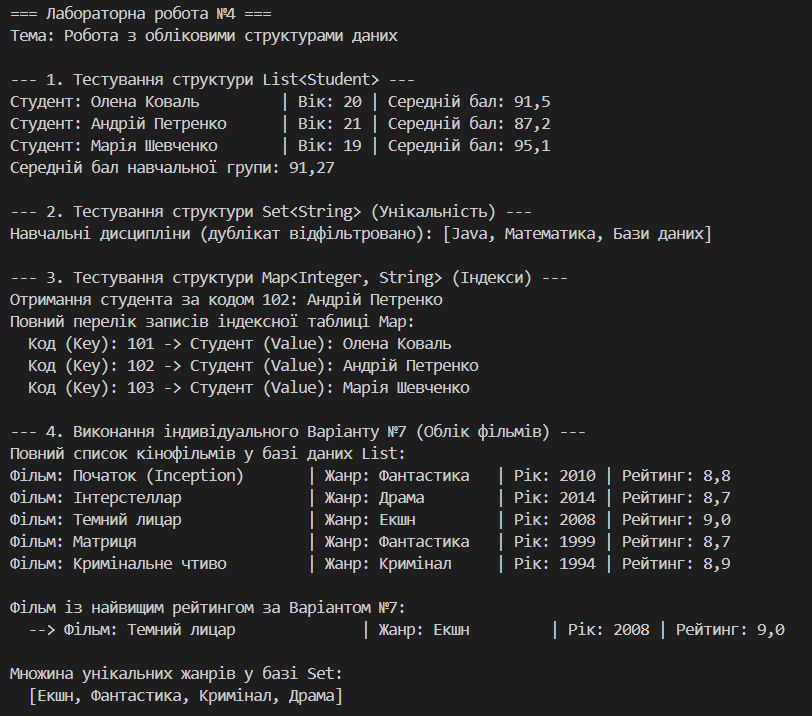
\includegraphics[width=0.95\textwidth]{screenshots/terminal_output.png}
    \caption{Вигляд терміналу після успішного виконання всіх чотирьох розділів Лабораторної роботи №4}
    \label{fig:terminal_lab4}
\end{figure}

На основі отриманих даних терміналу (рис.~\ref{fig:terminal_lab4}) проведено детальний 
покроковий аналіз результатів перевіірки колекцій:
\begin{enumerate}
    \item \textbf{Тестування динамічних списків (\texttt{List<Student>}):}
    Програма успішно ініціалізувала колекцію об'єктами трьох студентів. 
    На основі методу \texttt{size()} було автоматично вираховано точний середній 
    бал навчальної групи, який склав \texttt{91.27}. Порядок додавання елементів 
    зберігся без викривлень.
    
    \item \textbf{Тестування захисту від дублювання (\texttt{Set<String>}):}
    При спробі повторного надсилання ідентифікатора \texttt{"Java"} внутрішній 
    механізм \texttt{HashSet} заблокував створення копії. У консоль було виведено 
    чисту множину з трьох унікальних дисциплін, що повністю підтвердило закладені 
    в теорії правила унікальності.
    
    \item \textbf{Тестування індексної таблиці відображень (\texttt{Map}):}
    Впровадження структури \texttt{HashMap} дозволило виконати швидкий пошук за 
    ключем-кодом \texttt{102}, миттєво повернувши об'єкт рядка \texttt{"Андрій Петренко"}. 
    Повний перебір пар через \texttt{entrySet()} продемонстрував безпомилковий зв'язок 
    між первинними ключами та значеннями.
    
    \item \textbf{Аналіз індивідуального завдання Варіант №7 (Кінокаталог фільмів):}
    Сервісний менеджер \texttt{MovieManager} успішно проітерував список \texttt{List<Movie>}. 
    Програма безпомилково розрахувала лідера рейтингу — фільм \textbf{«Темний лицар»} із 
    максимальною оцінкою у \textbf{\texttt{9.0}} балів. Паралельно, завдяки 
    структурі \texttt{Set<String>}, було автоматично сформовано та виведено унікальну 
    множину жанрів: \texttt{[Фантастика, Кримінал, Драма, Екшн]}. Дублікат жанру «Фантастика» 
    для фільму «Матриця» було успішно відфільтровано «на льоту».
\end{enumerate}
